\documentclass{article}
\usepackage[utf8]{inputenc}

\title{TT3010 - Audio technology and room acoustics. \newline Exercise 7 - Music instruments.}


%\author{Jan Arne Bosnes}
\date{\today}

\usepackage{natbib}
\usepackage{graphicx}
\usepackage{multicol}
\usepackage{gensymb}
\usepackage{float}
\usepackage{wasysym}


\begin{document}

\maketitle

All tasks are based on chapters 10-12 in Rossings "Science of Sound" \cite{rossing}. 
It is recommended that the student will try to do every task, but tasks marked \textit{Mandatory} are to be handed in for approval (online). Deadline is November 6th.

\section*{Tasks}
%\begin{multicols}{2}
  {\bf \Large String instruments}
\begin{itemize}
    %\item [1.] Continue the sketches in fig. 10.4. to show the shape of the plucked string during the next half cycle from $t = \frac{1}{2} T$ to $t = T$.
  
    \item[1.] \textit{Mandatory.} In fig. 10.3. and 10.5, note that plucking a string one-fifth the distance from one end suppresses the fifth harmonic, and plucking it at the midpoint (one-half the distance) suppresses the second harmonic. Also note that the phase of the harmonics (indicated by + and -) changes in going through a zero. Using this information, draw a similar diagram to show the addition of modes  to obtain the shape of a string plucked at one-third its length.
    
    %\item[3.] Assuming a frequency of 440 Hz and a bow speed of 0.2 m/s in fig. 10.7, what is the displacement of the string at its midpoint? What is the speed of the string when it leaves the bow and "snaps" back? (\textit{Hint}: First determine the time during which the string moves at the speed of the bow.)

    %\item[4.] Note the similarity between the Chladni patterns in fig. 10.16 and the holograms in fig. 10.17 for modes II and V. Sketch a Chladni pattern that one might expect for mode I in figure 10.17.
    
    %\item[5.] If the main resonances (A and T in fig. 10.19) of the alto violin in the new family of fiddles are scaled to those of the conventional violin, near what notes will they lie? (The alto is tuned a fifth below the violin.) Compare these resonances to those of the viola.
     
    \item[2.] Determine the musical intervals between the strings of the guitar (see section 10.9) and those of the electric bass (see section 10.15).

\end{itemize}


  {\bf \Large Wind instruments}

\begin{itemize}
    
    \item[3.] \textit{Mandatory.} Calculate the two lowest resonance frequencies of a pipe 46 cm long closed at both ends. Do the same for a pipe 33 cm long. Now compare these frequencies to those given for the resonances $A_2$ and $A_4$ (longer pipe) and $A_3$ and $A_5$ (shorter pipe) in fig. 10.27c. Discuss the significance of the similarity.
 
%    \item[8.] Carefully measure the distance of each fret of a guitar from the saddle of the bridge, and determine how closely the rule of eighteen has been followed. If done carefully, you can determine how much compensation is included for each string. 
    
%     \item[4.] Calculate the frequencies of the first three resonances of closed tubes having length of 275 and 375 cm. Compare these to the resonances shown in the impedance curves of the French horn trombone.
    
%    \item[3.] Determine the frequencies of the trumpet resonances as accurately as you can from fig. 11.7. How closely do they correspond to the bugle notes: B$^\flat_3$, F$^\flat_4$, B$^\flat_4$, D$_5$, F$_5$, A$^\flat_5$ and B$^\flat_5$ (written C$_4$, G$_4$, E$_5$, G$_5$, B$^\flat$ and C$_6$)?

 %   \item[4.] Pressing the first valve of a trumpet or tuba increases the acoustic length by 12.2 \% and lowers the pitch a whole tone. How long must the first valve slide be in each of these instruments? (In other words, how many cm of tubing should be added to produce the pitch change?) If possible, compare your answers to the measured lengths in actual instruments.
    
  %  \item[5.] Find the frequency ratios of the first five peaks in fig. 11.4 to the corresponding peaks in fig. 11.6.
    
     \item [4.] \textit{Mandatory.} Assume that the length of a trombone is 275 cm in first ("open") position. How far should the slide have to be moved to lower the pitch one semitone? (Remember the length is increased by twice this amount.) If possible, compare this with the slide motion of an actual trombone.
   
       \item [5.] \textit{Mandatory.} A B$^\flat$ clarinet is about 67 cm long.
        \begin{itemize}
            \item[a.] What is the lowest resonance frequency of a closed pipe of that length?\footnote{In the book "Science of sound", the term "closed pipe" should be understood as a pipe which is closed at one end but open at the other end.}
            \item[b.] The lowest note on a B$^\flat$ clarinet is D$_3$. Compare its frequency to your answer in a.
            \item[c.] Can you explain the difference between these two frequencies?
        \end{itemize}
 
  \item[6.] The length of an alto recorder (from the wind-way to the bell) is about  42 cm.
        \begin{itemize}
            \item[a.] What are the lowest resonance frequency of an open pipe of that length?
            \item[b.] The lowest note on the recorder is $F_4$. Compare its frequency to your answer in a.
            \item[c.] Explain the difference between  these  two frequencies.
        \end{itemize}

%\item[8.] The length of a flute (from the embouchure hole to  the open end) is about 60 cm. What do you expect the frequency of the lowest note  to be?



\end{itemize}

%\end{multicols}

\begin{figure}[H]
    \centering
    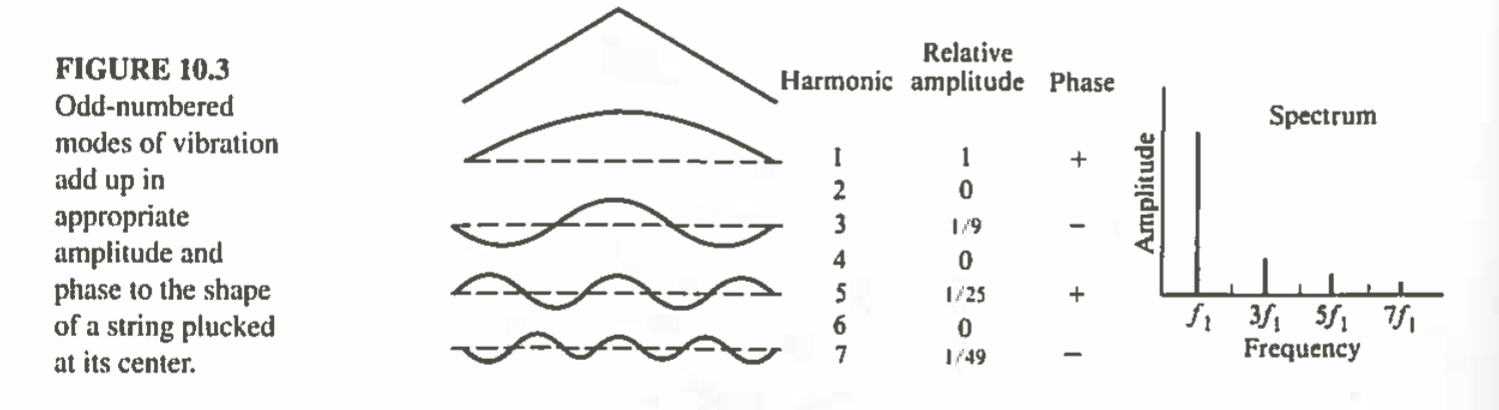
\includegraphics[scale = 0.8]{figures/fig10_3.png}
\end{figure}

\begin{figure}[H]
    \centering
    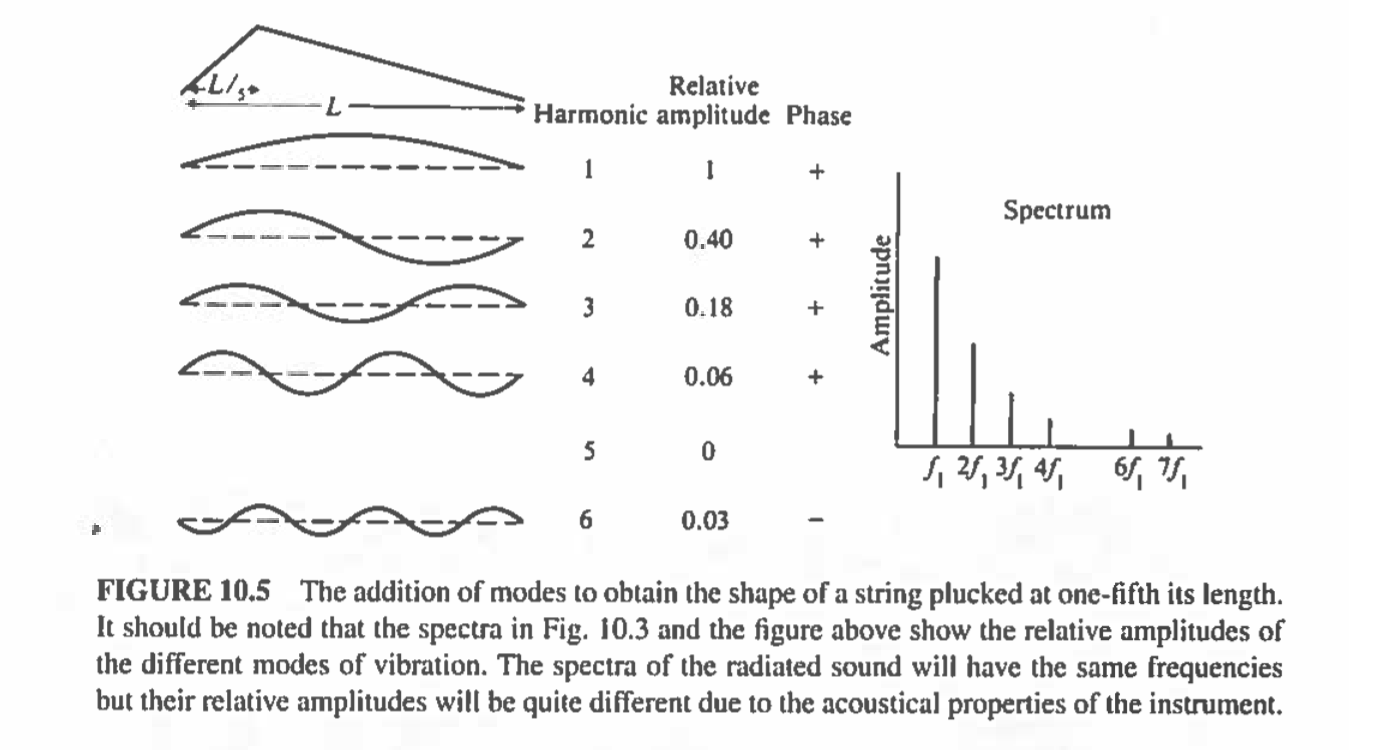
\includegraphics[scale = 0.8]{figures/fig10_5.png}
\end{figure}

\begin{figure}[H]
    \centering
    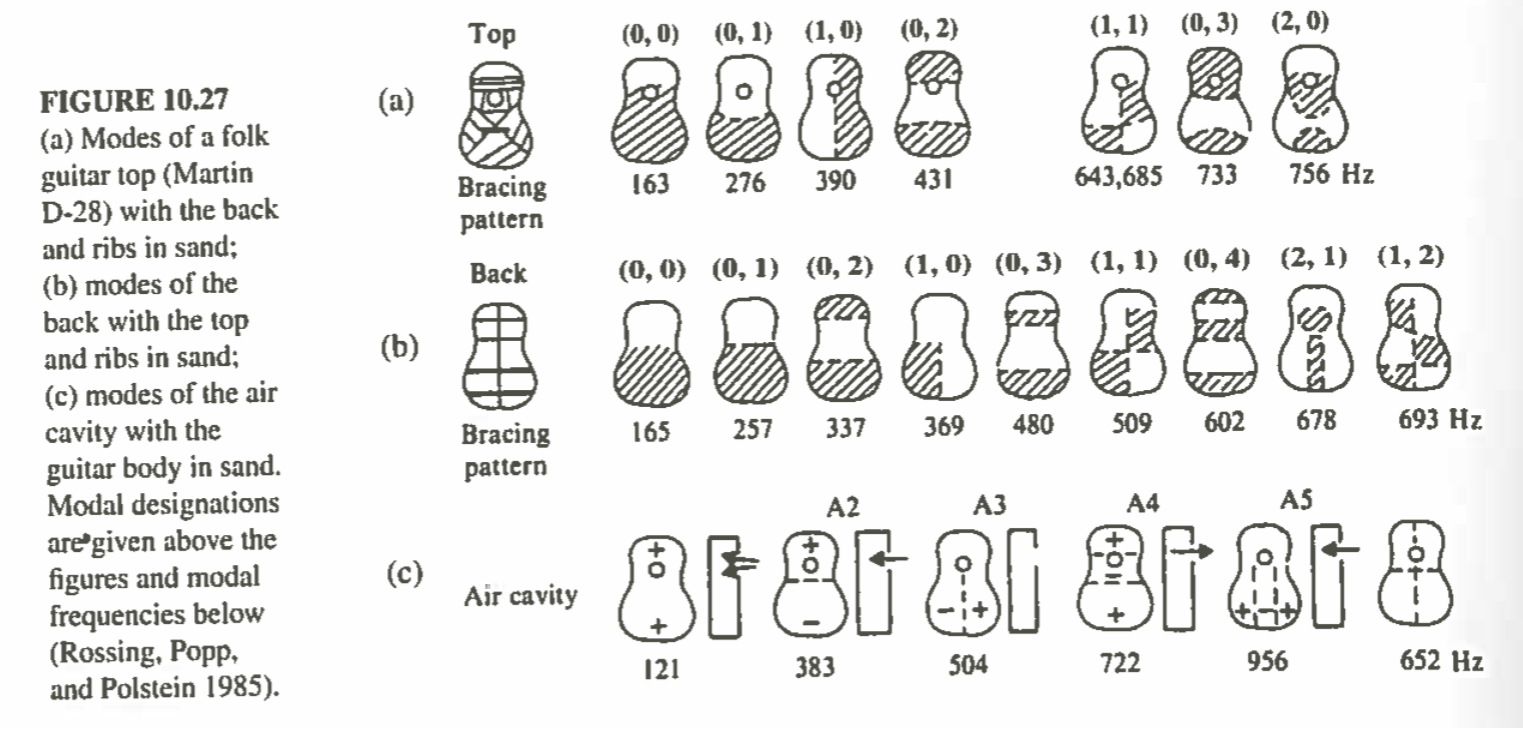
\includegraphics[scale = 0.8]{figures/fig10_27.png}
\end{figure}

\end{document}

